\chapter{Mogelijke uitbreidingen} \label{uitbreidingen}
Het eindresultaat van onze module is een afgerond geheel en is dus ook bruikbaar. Er zijn echter nog enkele mogelijk uitbreidingen die wij voor ogen zagen. Deze hebben wij niet ge\"{i}mplementeerd wegens tijdsgebrek. We sommen in dit hoofdstuk enkele van deze uitbreidingen op en hoe wij ze eventueel zouden implementeren.

\section{Keuze interval bij automatisch ophalen}
Onze huidige module voorziet een alternatieve vorm van de CoAP observe voor CoAP resources die niet observable zijn. Een gebruiker kan namelijk waarden periodiek laten ophalen, dit gebeurt aan de hand van opeenvolgende GET requests waartussen een bepaald interval ligt. In onze module bedraagt die een hardgecodeerd aantal seconden (namelijk 5). Men zou echter de module gebruiksvriendelijker en meer configureerbaar kunnen maken door de gebruiker het interval te laten kiezen. Dit zou gelijkaardig kunnen gebeuren aan de keuze van het polling interval, eerder besproken in paragraaf \ref{rest}.

\section{Opvragen devices in subnetwerk met resource directory}
Eerder werd al uitgelegd hoe resource discovery in zijn werk gaat. Men kan dit principe doortrekken op subnetwerkniveau. Wanneer op een subnetwerk een resource directory voorzien is kunnen embedded devices er hun well-known/core's in plaatsen. De module zou dan de gebruiker een lijst kunnen presenteren die alle aanwezige devices in het subnetwerk opsomt, samen met de aangesloten resources. Men zou ook hier weer modulair kunnen werken en de devices voorstellen als instanties van het content type CoAP device.\\

Nog een ander mogelijk alternatief dat overwogen werd is het sturen van een broadcast op het subnetwerk. Deze broadcast bevat dan een GET request die de well-known/core opvraagt van elk embedded device in het subnetwerk. Het nadeel bij deze benadering is dat een broadcast zeer belastend is voor het subnetwerk. Bovendien is het niet de bedoeling dat als een gebruiker ge\"{i}nteresseerd is in een ander subnetwerk, dat die belasting zomaar kan worden uitgevoerd.\\
Wanneer men echter gebruik maakt van een resource directory kan men bovendien beslissen welke embedded devices publiek worden gemaakt, wat de beveiliging en belasting van het subnetwerk ten goede komt.

\section{Conditional observe}
Het principe van een conditional observe is een uitbreiding van de standaard CoAP observe. Het werd mede ontwikkeld door iMinds en wordt omschreven in een aparte draft, namelijk de CoAP Conditional Observe draft (huidig versie 3).\\

Een conditional observe werkt net als een gewone CoAP observe met dat verschil dat een waarde pas naar de client wordt opgestuurd wanneer de waarde aan een bepaalde voorwaarde voldoet. Dit kan bijvoorbeeld een temperatuur zijn waarvan je pas op de hoogte wilt komen wanneer die hoger wordt dan 20 graden Celsius.\\
Voor de conditional observe wordt optie nummer 18 gebruikt. Deze optie moet steeds vergezeld worden van een gewone observe optie (nr. 6) aangezien deze er een extensie van is.

\begin{figure}[h!]
\label{fig:conditional}
\centering
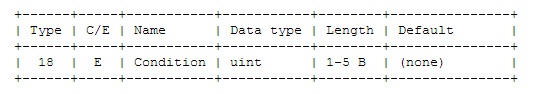
\includegraphics[width=0.8\textwidth]{fig/conditional}
\caption{Conditional observe optie (nr. 18)}
\end{figure}

De waarde kan vari\"{e}ren in lengte van \'{e}\'{e}n tot vijf bytes en bestaat uit de volgende onderdelen:

\begin{itemize}
\item TYPE: Beschrijft het type van de voorwaarde, bijvoorbeeld groter dan, kleiner dan, is gelijk aan,...
\item R: In een request duidt deze bit aan of de client de notificaties als confirmable (1) of non-confirmable (0) verkiest. In een response duidt deze bit aan of de server bereid is om in te gaan op het verzoek van de client om het betreffende soort berichten te sturen.
\item V: Deze twee bits duiden aan wat het type van de voorwaarde is (Integer, tijdsduur in seconden of float).
\item VAL: De waarde van de voorwaarde, de lengte hiervan kan vari\"{e}ren van 1 tot 4 bytes.
\end{itemize}

\begin{figure}[h!]
\label{fig:conditionalFormat}
\centering
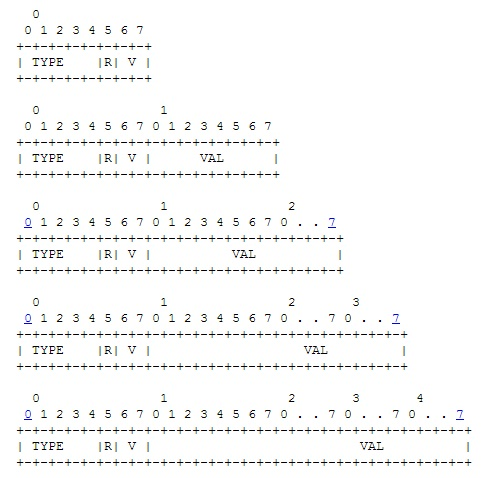
\includegraphics[width=0.8\textwidth]{fig/conditional_format}
\caption{Conditional observe optie formaat }
\end{figure}

\subsection{Keep-alive}
Men kan gebruik maken van de Keep-alive optie om er zeker van te zijn dat de client nog deel uitmaakt van de lijst van observers. Het betreft hier optie 30.

\begin{figure}[h!]
\label{fig:keepAlive}
\centering
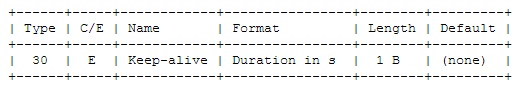
\includegraphics[width=0.8\textwidth]{fig/keep_alive}
\caption{De Keep-alive optie met nummer 30}
\end{figure}

Wanneer een client een Keep-alive optie meestuurt, vraagt die aan de server te bevestigen dat de client nog tot de lijst van observers behoort. En dit telkens wanneer een bepaald interval, meegegeven door de client in de optie, verstrijkt en er in dat interval geen notificaties of enkel non-confirmable berichten ontvangen zijn. De server stuurt dan een leeg bericht op, de voorwaarde werd immers niet voldaan.

\section{Drupal Entities}